\documentclass[pscyr]{hedlab}
\usepackage[russian]{babel}
\usepackage{graphicx}
\graphicspath{{images/}}
\usepackage{listings}

\lstset{
    basicstyle=\footnotesize,
    inputencoding=utf8,
    extendedchars=True,
    language=[Sharp]C,
    numbers=left,
    numberstyle=\footnotesize,
    breakatwhitespace=\false,
    breaklines=True,
    tabsize=2,
    keepspaces=true,
}

\labname{Использование хранимых процедур в Web-приложениях}
\labnum{5}
\student{Чечеткин И. А., САПР-1.1п}
\labdate{}

\begin{document}
    \makeheader
    \emph{Цель:} получение практических навыков создания хранимых процедур на
      MS SQL Server и реализации, вызов процедур из ASP.NET приложения.\\
    \emph{Задачи:} 
    \begin{enumerate}
        \item Создать базу данных согласно заданию.
        \item Реализовать не менее 3-х хранимых процедур, согласно заданию.
        \item Создать ASP.NET приложение, в котором осуществить вызов хранимых процедур.
    \end{enumerate}
    Реализация хранимых процедур:
    \lstinputlisting{code/code.cs}
    Вызов хранимых процедур:
    \lstinputlisting[inputencoding=koi8-r,language=HTML]{code/page.aspx}
    Хранимые процедуры:
    \lstinputlisting[language=SQL]{code/sql.sql}
    
    \pagebreak

    Скриншоты с Web-страниц:
    \begin{figure}[h!]
        \center
        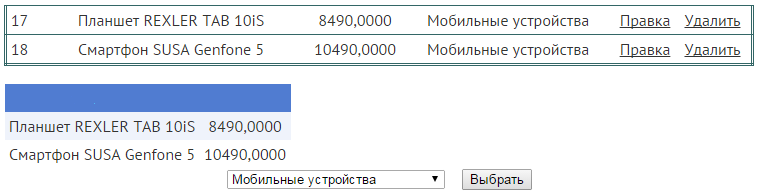
\includegraphics[width=.8\textwidth]{good_group} \\
        Реализация процедуры SelectGoods \\
        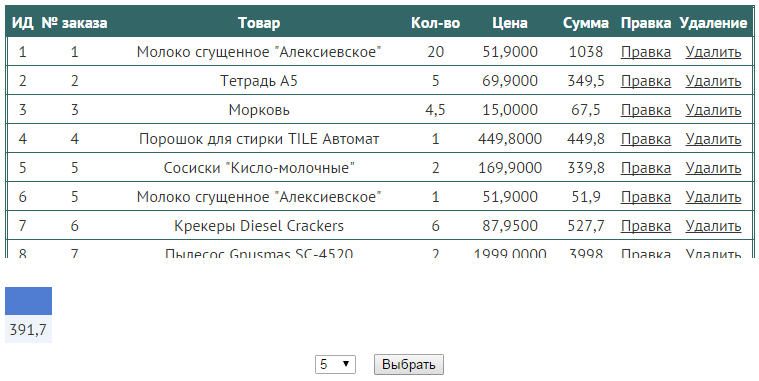
\includegraphics[width=.8\textwidth]{order_sum} \\
        Реализация процедуры OrderFullSum \\
        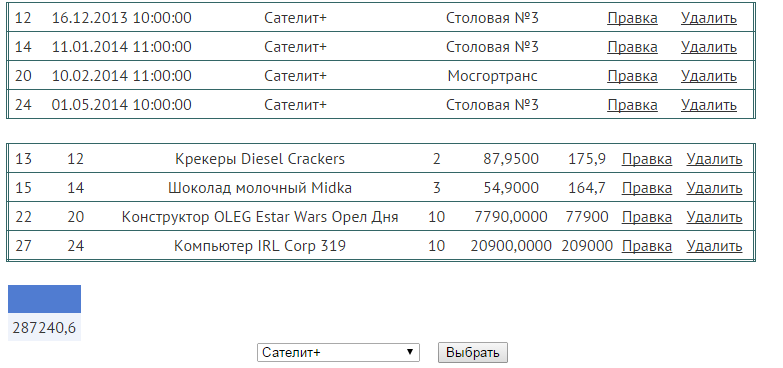
\includegraphics[width=.8\textwidth]{seller_sum} \\
        Реализация процедуры SellerOrdersSum
    \end{figure}

    \emph{Вывод:} в результате проделанной работы
    \begin{enumerate}
        \item Создал базу данных согласно заданию.
        \item Реализовали не менее 3-х хранимых процедур, согласно заданию.
        \item Создал ASP.NET приложение, в котором осуществить вызов хранимых процедур.
    \end{enumerate}
\end{document}